در ادامه هر یک از روش‌ها را جدا توضیح می‌دهیم:

\subsubsection*{TCP-Scanning}

در این روش، اسکنر تلاش می‌کند اتصال کامل TCP را با پورت مقصد برقرار کند. یعنی ابتدا بسته‌ی SYN ارسال می‌شود، اگر پورت باز باشد SYN-ACK برمی‌گردد، و سپس ACK ارسال می‌شود تا اتصال کامل شود.

مزایا:
\begin{itemize}
    \item بسیار دقیق است. وقتی ارتباط کامل برقرار شد، کاملاً مطمئن هستید که پورت باز است.
\end{itemize}

معایب:
\begin{itemize}
    \item بسیار راحت توسط سیستم مقصد شناسایی می‌شود (در لاگ‌ها ثبت می‌شود).
    \item نسبت به روش‌های دیگر کندتر است.
    \item به راحتی فایروال جلوی آن را می‌تواند بگیرد
\end{itemize}

\subsubsection*{SYN-Scanning}

در این روش، فقط بسته‌ی SYN ارسال می‌شود. اگر پورت باز باشد، SYN-ACK پاسخ داده می‌شود، ولی اسکنر دیگر ACK نمی‌فرستد و اتصال را نیمه‌کاره رها می‌کند.

مزایا:

\begin{itemize}
    \item سریع‌تر از TCP Scanning است.
    \item در لاگ‌های سیستم هدف کمتر دیده می‌شود.
\end{itemize}

معایب:

\begin{itemize}
    \item ممکن است توسط فایروال‌ها یا IDS/IPS ها مسدود شود.
\end{itemize}


\subsubsection*{FIN-Scanning}

در این روش، بسته‌ی FIN به پورت مقصد ارسال می‌شود. اگر پورت بسته باشد، دستگاه پاسخ RST می‌دهد. اگر باز باشد، هیچ پاسخی نمی‌دهد (بر اساس استاندارد TCP).

مزایا:

\begin{itemize}
    \item می‌تواند از بعضی فایروال‌ها عبور کند
\end{itemize}

معایب:

\begin{itemize}
    \item روی سیستم‌های ویندوز اغلب کار نمی‌کند، چون ویندوز به بسته FIN پاسخ RST می‌دهد حتی اگر پورت باز باشد.
    \item قابل اطمینان نیست مگر در سیستم‌های خاص ( مثل Unix/Linux ).
\end{itemize}


\subsubsection*{UDP-Scanning}

در این روش، بسته UDP به پورت ارسال می‌شود. اگر پورت بسته باشد، معمولا پیام ICMP-Port-Unreachable برمی‌گردد. اگر باز باشد، معمولا پاسخی دریافت نمی‌شود.

مزایا:

\begin{itemize}
    \item تنها روش کاربردی برای شناسایی پورت‌های باز UDP
\end{itemize}

معایب:

\begin{itemize}
    \item سخت‌ترین روش برای تشخیص وضعیت واقعی (باز یا بسته).
    \item کند است چون نیاز به تایم‌اوت دارد.
    \item ممکن است توسط فایروال‌ها مسدود شود.
\end{itemize}


\subsubsection*{جمع‌بندی موارد:}

\begin{itemize}
    \item TCP
    دقیق و کند و آشکار
    \item SYN
    سریع و نیمه مخفی
    \item FIN
    مخفی‌تر ولی کمتر قابل اطمینان
    \item UDP
    تنها راه برای بررسی UDP ولی کند و غیرقابل پیش‌بینی
\end{itemize}



ابتدا فایل داده شده را در نرم‌افزار Wireshark باز می‌کنیم و سپس در تب analyze و بخش display filters تعدادی رکورد برای شناسایی پورت‌های داد هشده اضافه می‌کنیم.

{
	
\centering{

	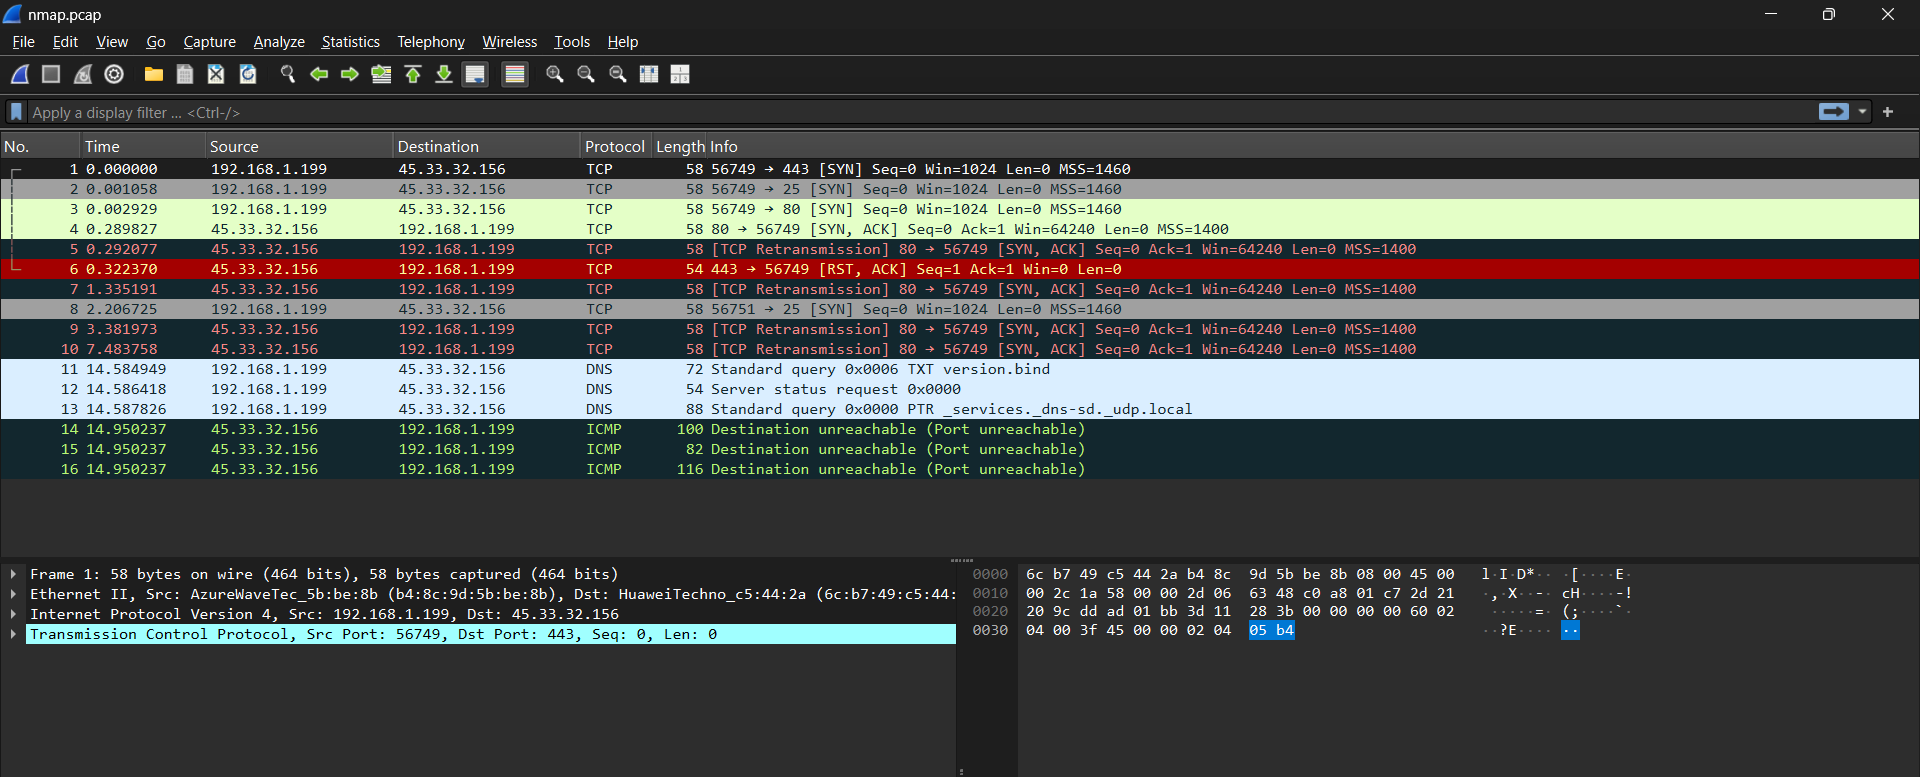
\includegraphics[width=0.9\linewidth]{screenshot002}

}

}

\textbf{پورت 25:}
با توجه به فریم 2 و 8 و اینکه هیچ پاسخی از سرور نیامده است، پس این پورت Filterd است.

\textbf{پورت 80:}
با توجه به فریم 3 و 4 و 5 و 7 این پورت Open است.

\textbf{پورت 443:}
با توجه به فریم 1 و 6 این پورت Closed است. چون که فلگ بسته RST فرستاده است.

\textbf{پورت 53:}
با توجه به فریم 11 و 12 و13 و 14 و 16 ، این پورت Closed است.  چون که در بسته ICMP کد 3 داده که یعنی Port Unreachable .